\documentclass[tikz,border=8pt]{standalone}
\usepackage[T1]{fontenc}
\usepackage{lmodern}
\usetikzlibrary{positioning,arrows.meta,calc,shapes.geometric}
\definecolor{nuevo}{RGB}{220,110,10}
\definecolor{nuevofill}{RGB}{255,236,214}
\definecolor{base}{RGB}{50,80,140}
\definecolor{basefill}{RGB}{226,234,248}
\definecolor{regc}{RGB}{110,110,110}
\begin{document}
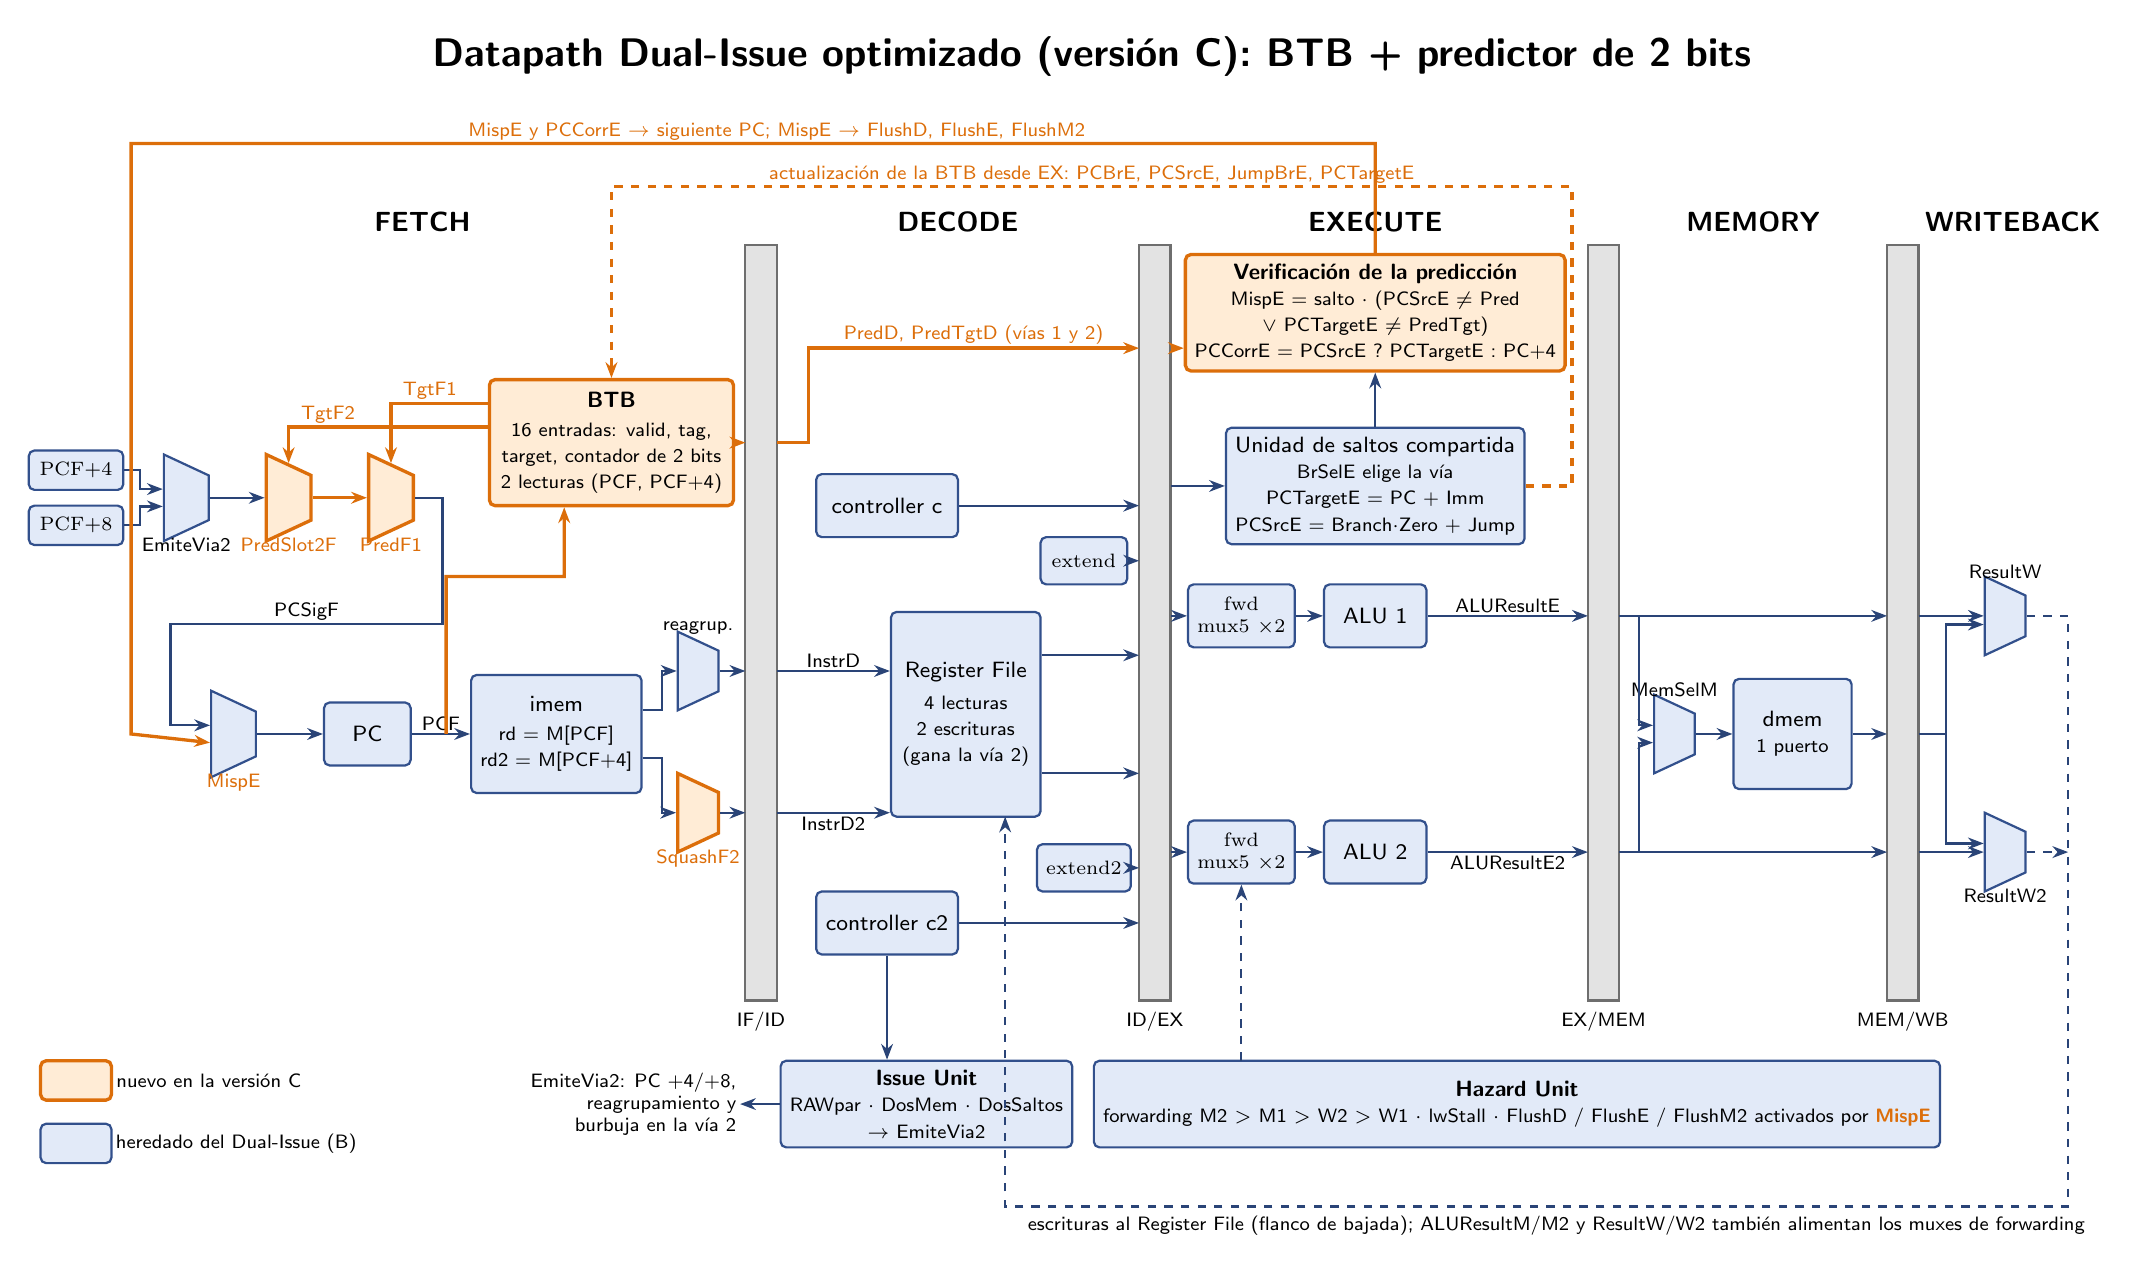
\begin{tikzpicture}[
  font=\sffamily\footnotesize,
  >={Stealth[length=2mm]},
  blk/.style={draw=base, fill=basefill, thick, rounded corners=2pt, align=center, minimum height=8mm, minimum width=16mm},
  nb/.style={draw=nuevo, fill=nuevofill, very thick, rounded corners=2pt, align=center, minimum height=8mm, minimum width=16mm},
  mux/.style={draw=base, fill=basefill, thick, trapezium, trapezium angle=65, shape border rotate=270, minimum width=11mm, minimum height=3.5mm, inner sep=1pt},
  nmux/.style={mux, draw=nuevo, fill=nuevofill, very thick},
  preg/.style={draw=regc, fill=gray!22, thick, minimum width=4mm, minimum height=96mm, anchor=south},
  lbl/.style={font=\sffamily\scriptsize, inner sep=1pt},
  nl/.style={lbl, text=nuevo},
  w/.style={->, thick, draw=base!85!black},
  nw/.style={->, very thick, draw=nuevo},
  fb/.style={->, thick, draw=base!85!black, dashed},
]

\node[font=\sffamily\bfseries\Large] at (9.5,12.0) {Datapath Dual-Issue optimizado (versión C): BTB + predictor de 2 bits};

\foreach \x/\n in {5.3/{IF/ID}, 10.3/{ID/EX}, 16.0/{EX/MEM}, 19.8/{MEM/WB}} {
  \node[preg] at (\x,0) {};
  \node[lbl] at (\x,-0.25) {\n};
}
\node[font=\sffamily\bfseries] at (1.0,9.9) {FETCH};
\node[font=\sffamily\bfseries] at (7.8,9.9) {DECODE};
\node[font=\sffamily\bfseries] at (13.1,9.9) {EXECUTE};
\node[font=\sffamily\bfseries] at (17.9,9.9) {MEMORY};
\node[font=\sffamily\bfseries] at (21.2,9.9) {WRITEBACK};

\node[blk, minimum width=11mm] (pc) at (0.3,3.4) {PC};
\node[mux] (mmisp) at (-1.4,3.4) {};
\node[nl, below=1pt of mmisp] {MispE};
\node[blk, minimum width=19mm, minimum height=15mm] (imem) at (2.7,3.4) {imem\\[1pt]\scriptsize rd = M[PCF]\\\scriptsize rd2 = M[PCF+4]};

\node[blk, minimum width=12mm, minimum height=5mm, font=\scriptsize] (a4) at (-3.4,6.75) {PCF+4};
\node[blk, minimum width=12mm, minimum height=5mm, font=\scriptsize] (a8) at (-3.4,6.05) {PCF+8};
\node[mux] (mseq) at (-2.0,6.4) {};
\node[lbl, below=1pt of mseq] {EmiteVia2};
\node[nmux] (mp2) at (-0.7,6.4) {};
\node[nl, below=1pt of mp2] {PredSlot2F};
\node[nmux] (mp1) at (0.6,6.4) {};
\node[nl, below=1pt of mp1] {PredF1};
\draw[w] (a4.east) -- ++(0.2,0) |- ([yshift=1.1mm]mseq.west);
\draw[w] (a8.east) -- ++(0.2,0) |- ([yshift=-1.1mm]mseq.west);
\draw[w] (mseq.east) -- (mp2.west);
\draw[nw] (mp2.east) -- (mp1.west);

\node[nb, minimum width=31mm, minimum height=16mm] (btb) at (3.4,7.1) {\textbf{BTB}\\[1pt]\scriptsize 16 entradas: valid, tag,\\\scriptsize target, contador de 2 bits\\\scriptsize 2 lecturas (PCF, PCF+4)};
\draw[nw] ([yshift=5mm]btb.west) -| node[nl, pos=0.3, above]{TgtF1} (mp1.north);
\draw[nw] ([yshift=2mm]btb.west) -- ++(-1.6,0) node[nl, pos=0.5, above]{} -| (mp2.north);
\node[nl] at (-0.2,7.45) {TgtF2};

\draw[w] (mp1.east) -- ++(0.35,0) |- node[lbl, pos=0.75, above]{PCSigF} (-2.2,4.8) |- ([yshift=1.1mm]mmisp.west);
\draw[w] (mmisp.east) -- (pc.west);
\draw[w] (pc.east) -- node[lbl,above]{PCF} (imem.west);
\draw[nw] (1.3,3.4) |- (2.8,5.4) -- ([xshift=-6mm]btb.south);

\node[mux, minimum width=10mm] (rg) at (4.5,4.2) {};
\node[lbl, above=1pt of rg] {reagrup.};
\node[nmux, minimum width=10mm] (sq) at (4.5,2.4) {};
\node[nl, below=1pt of sq] {SquashF2};
\draw[w] ([yshift=3mm]imem.east) -- ++(0.25,0) |- (rg.west);
\draw[w] ([yshift=-3mm]imem.east) -- ++(0.25,0) |- (sq.west);
\draw[w] (rg.east) -- (5.1,4.2);
\draw[w] (sq.east) -- (5.1,2.4);

\draw[nw] (btb.east) -- (5.1,7.1);
\draw[nw] (5.5,7.1) -- (5.9,7.1) |- (10.1,8.3);
\node[nl, above] at (8.0,8.3) {PredD, PredTgtD (vías 1 y 2)};

\node[blk, minimum width=18mm] (c1) at (6.9,6.3) {controller c};
\node[blk, minimum width=18mm] (c2) at (6.9,1.0) {controller c2};
\node[blk, minimum width=19mm, minimum height=26mm] (rf) at (7.9,3.65) {Register File\\[2pt]\scriptsize 4 lecturas\\\scriptsize 2 escrituras\\\scriptsize (gana la vía 2)};
\node[blk, minimum width=11mm, minimum height=6mm, font=\scriptsize] (ex1) at (9.4,5.6) {extend};
\node[blk, minimum width=11mm, minimum height=6mm, font=\scriptsize] (ex2) at (9.4,1.7) {extend2};
\draw[w] (5.5,4.2) -- node[lbl, above]{InstrD} (rf.west |- 0,4.2);
\draw[w] (5.5,2.4) -- node[lbl, below]{InstrD2} (rf.west |- 0,2.4);
\draw[w] (rf.east |- 0,4.4) -- (10.1,4.4);
\draw[w] (rf.east |- 0,2.9) -- (10.1,2.9);
\draw[w] (ex1.east) -- (10.1,5.6);
\draw[w] (ex2.east) -- (10.1,1.7);
\draw[w] (c1.east) -- (10.1,6.3);
\draw[w] (c2.east) -- (10.1,1.0);

\node[blk, minimum width=30mm, minimum height=11mm] (iu) at (7.4,-1.3) {\textbf{Issue Unit}\\\scriptsize RAWpar $\cdot$ DosMem $\cdot$ DosSaltos\\\scriptsize $\rightarrow$ EmiteVia2};
\draw[w] (c2.south) -- (c2.south |- iu.north);
\draw[w] (iu.west) -- ++(-0.5,0) node[lbl, left, align=right]{EmiteVia2: PC +4/+8,\\reagrupamiento y\\burbuja en la vía 2};

\node[blk, minimum width=13mm, font=\scriptsize] (f1) at (11.4,4.9) {fwd\\mux5 $\times$2};
\node[blk, minimum width=13mm, font=\scriptsize] (f2) at (11.4,1.9) {fwd\\mux5 $\times$2};
\node[blk, minimum width=13mm] (alu1) at (13.1,4.9) {ALU 1};
\node[blk, minimum width=13mm] (alu2) at (13.1,1.9) {ALU 2};
\draw[w] (10.5,4.9) -- (f1.west);
\draw[w] (10.5,1.9) -- (f2.west);
\draw[w] (f1) -- (alu1);
\draw[w] (f2) -- (alu2);
\draw[w] (alu1.east) -- node[lbl, above]{ALUResultE} (15.8,4.9);
\draw[w] (alu2.east) -- node[lbl, below]{ALUResultE2} (15.8,1.9);

\node[blk, minimum width=34mm, minimum height=12mm] (bu) at (13.1,6.55) {Unidad de saltos compartida\\\scriptsize BrSelE elige la vía\\\scriptsize PCTargetE = PC + Imm\\\scriptsize PCSrcE = Branch$\cdot$Zero + Jump};
\node[nb, minimum width=34mm, minimum height=11mm] (vf) at (13.1,8.75) {\textbf{Verificación de la predicción}\\\scriptsize MispE = salto $\cdot$ (PCSrcE $\neq$ Pred\\\scriptsize $\lor$ PCTargetE $\neq$ PredTgt)\\\scriptsize PCCorrE = PCSrcE ? PCTargetE : PC+4};
\draw[w] (10.5,6.55) -- (bu.west);
\draw[nw] (10.5,8.3) -- (vf.west |- 0,8.3);
\draw[w] (bu.north) -- (vf.south);
\draw[nw] (vf.north) -- (13.1,10.9) -| (-2.7,3.4) -- ([yshift=-1.1mm]mmisp.west);
\node[nl, above] at (5.5,10.9) {MispE y PCCorrE $\rightarrow$ siguiente PC; MispE $\rightarrow$ FlushD, FlushE, FlushM2};
\draw[nw, dashed] (bu.east) -- (15.6,6.55) |- (3.4,10.35) -- (btb.north);
\node[nl, above] at (9.5,10.35) {actualización de la BTB desde EX: PCBrE, PCSrcE, JumpBrE, PCTargetE};

\node[mux, minimum width=10mm] (mport) at (16.9,3.4) {};
\node[lbl, above=1pt of mport] {MemSelM};
\node[blk, minimum width=15mm, minimum height=14mm] (dm) at (18.4,3.4) {dmem\\\scriptsize 1 puerto};
\draw[w] (16.2,4.9) -- (19.6,4.9);
\draw[w] (16.2,1.9) -- (19.6,1.9);
\draw[w] (16.45,4.9) |- ([yshift=1.1mm]mport.west);
\draw[w] (16.45,1.9) |- ([yshift=-1.1mm]mport.west);
\draw[w] (mport) -- (dm);
\draw[w] (dm.east) -- (19.6,3.4);

\node[mux, minimum width=10mm] (wb1) at (21.1,4.9) {};
\node[mux, minimum width=10mm] (wb2) at (21.1,1.9) {};
\node[lbl, above=1pt of wb1] {ResultW};
\node[lbl, below=1pt of wb2] {ResultW2};
\draw[w] (20.0,4.9) -- (wb1.west);
\draw[w] (20.0,1.9) -- (wb2.west);
\draw[w] (20.0,3.4) -- (20.35,3.4) |- ([yshift=-1.1mm]wb1.west);
\draw[w] (20.35,3.4) |- ([yshift=1.1mm]wb2.west);
\draw[fb] (wb1.east) -- (21.9,4.9) |- (21.9,-2.6) -| (8.4,2.35);
\draw[fb] (wb2.east) -- (21.9,1.9);
\node[lbl] at (15.4,-2.85) {escrituras al Register File (flanco de bajada); ALUResultM/M2 y ResultW/W2 también alimentan los muxes de forwarding};

\node[blk, minimum width=64mm, minimum height=11mm] (hu) at (14.9,-1.3) {\textbf{Hazard Unit}\\\scriptsize forwarding M2 $>$ M1 $>$ W2 $>$ W1 $\cdot$ lwStall $\cdot$ FlushD / FlushE / FlushM2 activados por \textcolor{nuevo}{\textbf{MispE}}};
\draw[fb] (11.4,-0.75) -- (f2.south);

\node[nb, minimum width=9mm, minimum height=5mm, label={[lbl]right:nuevo en la versión C}] at (-3.4,-1.0) {};
\node[blk, minimum width=9mm, minimum height=5mm, label={[lbl]right:heredado del Dual-Issue (B)}] at (-3.4,-1.8) {};
\end{tikzpicture}
\end{document}
